\documentclass[11pt, oneside]{article}   	% use "amsart" instead of "article" for AMSLaTeX format
\usepackage{geometry}                		% See geometry.pdf to learn the layout options. There are lots.
\geometry{letterpaper}                   		% ... or a4paper or a5paper or ... 
%\geometry{landscape}                		% Activate for rotated page geometry
%\usepackage[parfill]{parskip}    		% Activate to begin paragraphs with an empty line rather than an indent
\usepackage{graphicx}				% Use pdf, png, jpg, or eps§ with pdflatex; use eps in DVI mode
								% TeX will automatically convert eps --> pdf in pdflatex		
\usepackage{amssymb}

\topmargin-3.3cm
\oddsidemargin-1.5cm
\evensidemargin-1.5cm
\textheight 10.8in
\textwidth 7.5in
%SetFonts

%SetFonts


\title{\sffamily Image quality stydy}
\date{}							% Activate to display a given date or no date

\begin{document}
\vspace{-0.5in}
\maketitle
\vspace{-0.5in}
\sffamily
The aim of the study you participated in, was to assess the rendering performance of displays with different dynamic ranges. The ensemble of scenes you saw, had a very high dynamic range, with maximal luminance in excess of 50,000 cd/m$^2$ and low luminance of around 0 cd/m$^2$. These scenes were rendered on two typical displays: (i) an LCD display, with a maximum luminance of 200 cd/m$^2$, and (ii) an OLED display, with a maximal luminance of 600 cd/m$^2$. For reference, the luminance of the sun at noon time is about 1.6 $\times$ 10$^9$ cd/m$^2$, whereas the luminance of the moon is around 2,500 cd/m$^2$.



To present scenes with such high dynamic ranges on these typical displays, their luminance had to be scaled down to the range that could be achieved by the employed displays. In video rendering technology, this scaling is called {\em tone mapping}. In high dynamic range scenes, a linear tone mapping function results in very dark images, as most of the scene content is mapped to near zero display luminances. A better tone mapping approach is to use compressive functions, in which low luminance levels are mapped linearly to display luminance, whereas higher luminance levels are progressively compressed. Examples of scene renderings with two different tone mapping methods are shown in Figure1.
 
 \begin{figure}[h] %  figure placement: here, top, bottom, or page
   \centering
   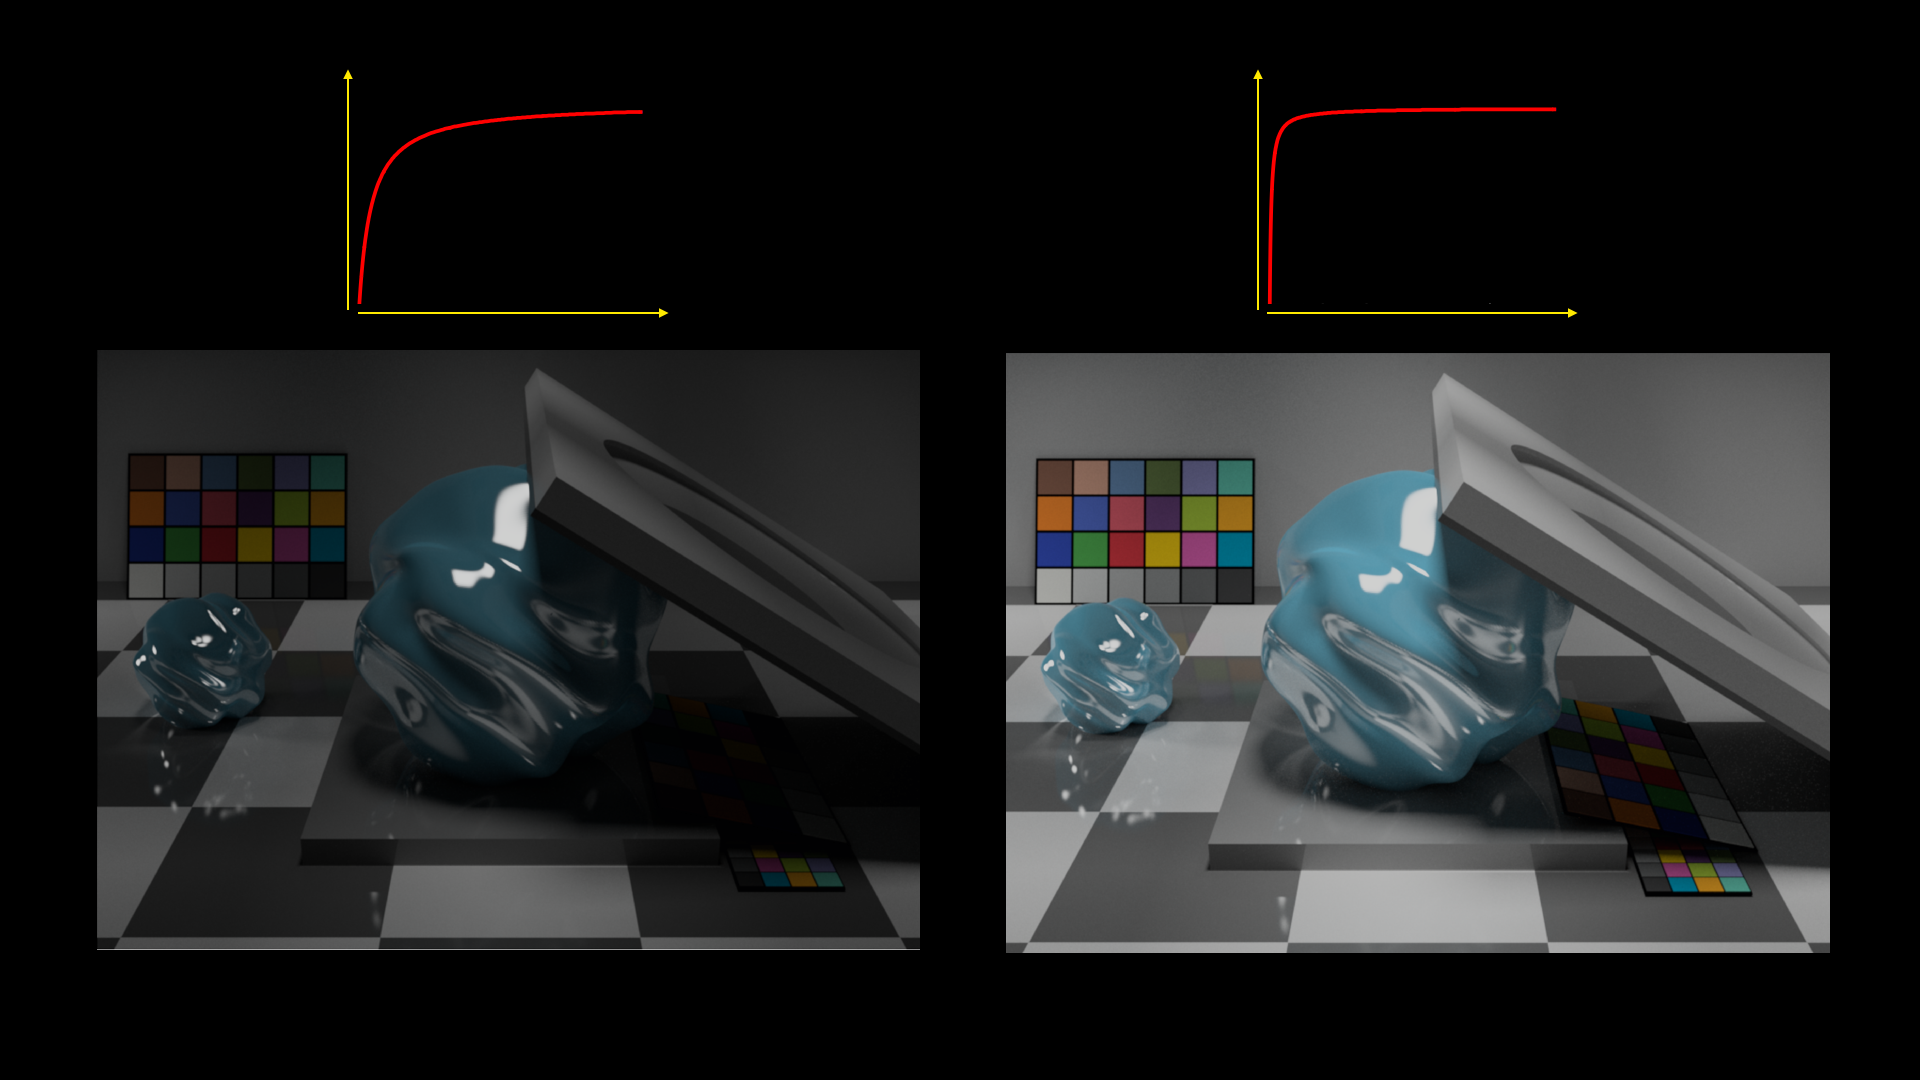
\includegraphics[width=7in]{ToneMappingExamples.png} 
   \caption{\sffamily \em Example tone mapping functions (top) and resulting images (bottom). The tone mapping functions (red lines) map scene luminance (x-axis) onto display luminance (y-axis). The less compressive function (left) maintains resolution of the highlights of the blobbie object, but results in a darker image overall. The more compressive function (right) results in a brighter image, but resolution of the highlights is lost, and the object material appears more 'plasticky'.}
   \label{fig:example}
\end{figure}

The data we collected on the first two sessions, were used to determine the optimal, for you, tone mapping functions separately for the two displays. Comparison of the two tone mapping functions can give insight into designing tone mapping functions for different displays with varying luminance ranges. The data we collected on the third session, were used to contrast the performance of the LCD vs. the OLED display and to determine the conditions (scenery and applied tone mapping) under which one display performs better (subjectively) than the other.\\

Thank you for your participation.

%\section{}
%\subsection{}



\end{document}  

 